\documentclass{article}

% Language setting
% Replace `english' with e.g. `spanish' to change the document language
\usepackage[english]{babel}

% Set page size and margins
% Replace `letterpaper' with `a4paper' for UK/EU standard size
\usepackage[letterpaper,top=2cm,bottom=2cm,left=3cm,right=3cm,marginparwidth=1.75cm]{geometry}

% Useful packages
\usepackage{amsmath}
\usepackage{graphicx}
\usepackage[colorlinks=true, allcolors=blue]{hyperref}
\usepackage{fancyhdr}
\usepackage{eurosym} % para el euro
\hyphenation{Re-a-li-za-das}
%\usepackage[pages=1]{background}
%\BgThispage
%\usepackage[paperwidth=12cm]{geometry}  
%\usepackage[dvipsnames]{xcolor} % To access some named colors used with \highLight
%\usepackage{luacolor} % Required to use the lua-ul \highLight command 
%\usepackage{lua-ul} 

\begin{document}
\begin{titlepage}
\centering
{\bfseries\LARGE I.E.S. Punta del Verde \par}
\vspace{1cm}
{\scshape\Large Desarrollo de aplicaciones Web \par}
\vspace{3cm}
{\scshape\Huge  KnowBuySell \par}
\vspace{3cm}
{\itshape\Large Proyecto Fin de Grado \par}
\vfill
{\Large Autor: \par}
{\Large Yolanda Morales Zamora \par}
\vfill
{\Large Junio 2024 \par}
\end{titlepage}


%\title{KnowBuySell}
%\author{Yolanda Morales Zamora\\I.E.S.Punta del Verde.}
%\maketitle

%\begin{abstract} 
%\end{abstract}

\section{Introduction}
%\href{https://www.overleaf.com/learn}{help library}, or head to our plans page to \href{https://www.overleaf.com/user/subscription/plans}{choose your plan}.
%Proyecto para el final de Grado Superior de Desarollo de Aplicaciones Web. 

\subsection{Introducción del proyecto}
%Breve introducción justificando los motivos para la elaboración del proyecto y/o necesidades en el sector productivo para la elaboración del mismo. Se pueden añadir también las ventajas que puede tener el uso del proyecto
Este proyecto se ha elaborado a raíz de la necesidad de control de información por parte de los usuarios de una plataforma de compras, para gestionar esa información para su mejor organización económica, es decir, como usuario "quiero saber en qué gasto más dinero o menos dinero" y a su vez con la misma información obtenida generar marketing personalizado para el usuario por parte de la entidad vendedora, es decir, como empresa "quiero conocer que es lo que más compra el usuario según cactegoría para ofrecerle otros productos que no conozca de la misma categoría" .\\

\textbf{Datos técnicos básicos del proyecto:}

\textbf{Nombre del proyecto:} Knowbuysell.

\textbf{Framework utilizado:} Laravel, el framework de los artesanos de la web.

\textbf{Lenguaje de programación:} PHP, Blade, Javascript.

Lenguaje Latex para la realización de este informe.

\subsection{Propósito}
%Especificar características del proyecto y uso una vez desarrollado.
Desarrollar una aplicación que ayude a mejorar el control económico del usuario cuando compre a través de ella, y a la misma vez,  ayude a mejorar el marketing de la entidad vendedora, a través de la información registrada. A través de la información registrada organizarla para beneficiar a la parte del "cliente" y a la parte del "servidor".

\subsection{Objetivos del proyecto}
%Esquema numerado de los objetivos de este proyecto que permitirá alcanzar el propósito que se ha especificado anteriormente.
%A modo de ejemplo se muestran los siguientes:
%1.- Realizar un estudio de los requisitos necesarios.
%2.- Desarrollo de aplicación que realizará la tarea de . .  .
%3.- Desarrollar una interfaz de uso sencilla e intuitiva
%4.- Redacción de los manuales de usuario e instalación
%5.- Redacción de la memoria del proyecto
Objetivos del proyecto:
\begin{itemize}
\item a) control por parte del usuario de la información que generan sus compras realizadas  
\item b) el control por parte de la entidad vendedora de la información de compra del cliente para ofrecerle más productos o servicios (mejora de marketing).

En los apartados a) y B) se reutiliza la misma información sólo que según el enfoque del cliente o servidor variará su gestión o uso.
\end{itemize}
\subsection{Coste del proyecto}
%Estimación del coste y esfuerzo del software y/ o hardware requerido para la realización del mismo. Podemos dividir en dos subapartados:
\subsubsection{Costes de desarrollo}
%Costes para la realización del sistema. Se dividen en Costes Recursos Informáticos (costes hardware y software) y Costes de personal.
Los costes directos comprenden los costes de personal. Para calcular el coste de personal es necesario saber cuál es el salario bruto del trabajador y los costes sociales. Para llevar a cabo esta planificación se tiene en cuenta un contrato a tiempo completo, en el que la empresa debe abonar una cuota patronal a la seguridad social del 23,60\% actualmente en España.

Estableciendo el coste medio de la hora por parte de un programador en España en 20 euros y siendo 500 las horas totales planificadas para el desarrollo del proyecto completo, se obtiene una remuneración total bruta de 10.000 euros. Tabla \ref{tab:my_labe_1}:


\begin{table}[htbp]
\centering
\begin{tabular}{|l|l|}
\hline
Concepto                & Coste    \\ \hline
Remuneración bruta      & 10.000 \euro \\ \hline
Costes Seguridad Social &  2.360 \euro \\ \hline
TOTAL                   & 12.360 \euro \\ \hline
\end{tabular}
 \caption{Costes directos}
    \label{tab:my_labe_1}
\end{table}

Para la obtención de los costes indirectos, en este caso, hay que tener en cuenta la amortización del equipo utilizado por el trabajador.\newline
La tabla \ref{tab:my_labe_3} muestra aquellos dispositivos hardware que están expuesto a un desgaste en el tiempo en el que se elabora el el proyecto:

\subsubsection{Costes de implantación}
%Costes para poner en funcionamiento el sistema. Resumen del coste total de ponerlo en funcionamiento
Debemos tener en cuenta que a continuación damos estimaciones de los costes de implantación:
\begin{itemize}

\item En cuanto a Hosting y Servidores:
        \subitem Hosting Compartido: 5 a 20 \euro/ mes
        \subitem Servidor VPS: 20 a 100 \euro/ mes
        \subitem Servidor Dedicado: 80 a 300 \euro/ mes
        \subitem Servicios en la Nube (AWS, Google Cloud, Azure): 50 a 200 \euro/mes

\item Para un primer mes de operación:
        \subitem Costo Inicial de Hosting: 50 a 300 \euro/ anual
        \subitem Registro de Dominio: 10 a 15 \euro/ anual 

\item Certificados SSL: 0 a 200 \euro/anual (Let's Encrypt gratuito o pagos de proveedores como Comodo)

Subtotal Infraestructura ((Primer Mes): 60 a 515 \euro 

\item Licencias y Herramientas
    \subitem IDE y Herramientas de Desarrollo:  utilizamos herramientias de código abierto y gratuitas como Viscual Studio Code a modo de IDE.
    Licencias de Software: Depende de necesidades específicas, pero generalmente bajo costo

Subtotal Licencias y Herramientas = 0 \euro
\item Seguridad y Auditorías
    \subitem Firewall y Seguridad en la Nube (opcional): 20 a 100 \euro /mes
    \subitem Auditorías de Seguridad: 500 a 1,500 \euro / mes

Subtotal Seguridad y Auditorías: 520 a 1,600 \euro / mes


\textbf{Total del importe estimado:
    \subitem Coste fijo: 12.360 \euro
    \subitem Coste variable: 580 a 2.115 \euro/ mes}
\end{itemize}

\section{Análisis del sistema}

\subsection{Introducción}

En este apartado detallamos el proyecto a realizar: análisis, diseño, implementación o codificación y prueba.

\subsection{Análisis de requisitos}
%Propósito último del proyecto, las propiedades que debe satisfacer y las restricciones a las que ha sido impuesto. Tras haber definido el propósito último del proyecto, el siguiente paso consiste en especificar los requerimientos (conjunto de propiedades o restricciones) del mismo, tanto funcionales como no funcionales.
El proyecto quiere obtener la mejora en la información económica registrada para el usuario de la aplicación así como la mejora a nivel de marketing para la empresa que presta el servicio de venta. El usuario debe poder realizar la compra de productos, descargar la información y crear un documento formato PDF, acceder a su registro, a la información de sus compras, poder comprar, modificar la compra y eliminar la compra. El usuario no podrá acceder a la información de otros usuarios, sólo a la suya propia.
El administrador o empleado de la empresa propietaria de la aplicación, podrá acceder a toda la información de las compras realizadas por cada usuario, podrá modificar, eliminar cualquier registro de la base de datos, podrá obtener la información en formato gráfica de las categorías de compras realizadas por el usuario con la finalidad de mejorar el marketing para poder aumentar la compras, y por tanto los beneficios.

%Como poner la referencia a una imagen\ref{fig:frog} 
%\Como poner enlace href{https://www.overleaf.com/learn/how-to/Including_images_on_Overleaf}{including images on Overleaf}.

\subsubsection{Requerimientos funcionales}
Los requisitos funcionales de una aplicación web son las funciones y características específicas que la aplicación debe tener para cumplir con los objetivos y necesidades de los usuarios.
En nuestro proyecto, aunque algunos no se hayan conseguido como metas serían los siguientes:\\
\begin{itemize}
    \item Inicio de sesión (Conseguido)
    \item Registro de usuario (Conseguido)
    \item Gestión de perfiles (Conseguido)
    \item CRUD para realizar compras (Conseguido)
    \item Integración de terceros como un sistema de pagos (No conseguido)
    \item Medidas de seguridad: cifrado de claves de usuario (Conseguido)
    \item Doble verificación (No conseguido)
\end{itemize}
% Qué son y cuales encuentras en tu proyecto.
\subsubsection{Requerimientos no funcionales}
Los requisitos no funcionales de una aplicación web son las características que definen la calidad y el comportamiento del sistema en lugar de las funciones específicas que realiza. En nuestro caso serían los siguientes:\\
\begin{itemize}
    \item Rendimiento: rapidez que se consigue con Laravel 
    \item Disponibilidad (No conseguido)
    \item Seguridad: autenticación, CSRF (Conseguido)
    \item Usabilidad: intuitiva y claridad en el diseño (Conseguido)
    \item Mantenibilidad: modularización del código a través de Modelo Vista Controlador, documentación (Conseguido)
    \item Cumplimiento Normativo: GDPR o Legislación de Protección de datos.
\end{itemize}
\subsection{Casos de uso: Diagramas y Narrativas de Caso de Uso}
% Explica que son estos diagramas y realiza los pertinentes para tu aplicación.
% https://ingsotfwarekarlacevallos.wordpress.com/2015/06/04/uml-casos-de-uso/
Los diagramas de casos de uso reflejarán las funcionalidades que correspondan a cada uno de los ámbitos concretos y más importantes del sistema. En la narrativa de los casos de uso se especifica las funciones, tareas e interacciones que se dan lugar en el sistema, es decir, se describen detalladamente cada uno de los casos de uso.
Lo habitual es realizar diagramas de tipo UML, nuestro diagrama conforme al proyecto, se puede comprobar en la \ref{fig:diaUML1} como se puede constatar más abajo.

Una vez observado el diagrama \ref{fig:diaUML1}, en nuestro caso, tenemos dos actores: \textbf{usuario} y \textbf{administrador}. El \textbf{usuario} gestionará las tareas indicadas en el diagrama, como son: registrar usuario, iniciar sesión, realizar compras a través de un CRUD, generar documentos en formato PDF de cada listad de compras y obtener información procentual de las compras en gráficas para saber en qué se gasta más el dinero y cómo progresa las compras de cada usuario; por otro lado como hemos indicado, tenemos a otro actor que es el \textbf{administrador} cuyas funciones consisten en: supervisar y gestionar las posibles incidencias de las tareas o actividades generadas por del usuario, y además extraer la información almacenada del usuario y con ella generar ofertas atractivas dirigidas al usuario. Es en la tarea de obtener información porcentual en gráficas la que ambos actores tienen un punto en común, pues la actividad que genera la información porcentual del usuario, es extraída por el administrador y gracias a esta información recopilada podrá generar ofertas que posteriormente irán dirigidas al usuario, con el fin de aumentar las ventas y obtener beneficios económicos en la empresa objeto de crean de esta aplicación web, tal y como hemos indicado.\\

DIAGRAMA DE CASO DE USO: APLICACIÓN WEB KNOWBUYSELL (Figura \ref{fig:diaUML1})

\begin{figure}[h]
\centering
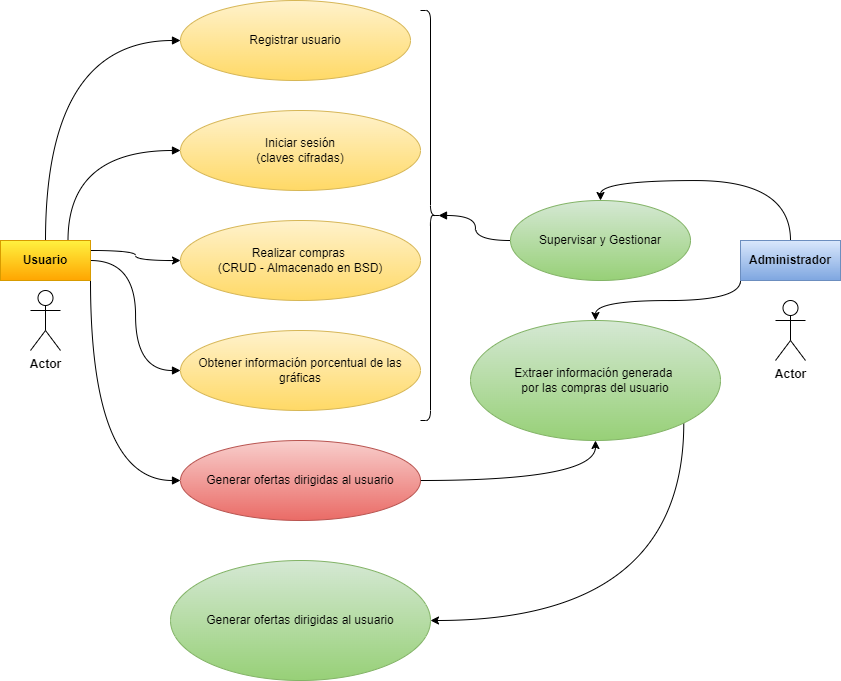
\includegraphics[scale=0.5]{Diagr_CUso.png}
\caption{\label{fig:diaUML1}Diagrama de la interacción en la aplicación web: Knowbuysell.}
\end{figure}

NARRATIVAS DE CASOS DE USO (Tablas \ref{tab:my_labe_2},\ref{tab:my_labe_3},\ref{tab:my_labe_4}, \ref{tab:my_labe_5}, \ref{tab:my_labe_6} y \ref{tab:my_labe_7})

% \begin{table}[]
% \centering
% \resizebox{\columnwidth}{!}{%
% \begin{tabular}{|l|l|}
% \hline
% \textbf{Referencia :} & CU-01 \\ \hline
% \textbf{Título del caso de uso:} & Registrar usuario \\ \hline
% \textbf{Actor:} & Usuario \\ \hline
% \textbf{Condiciones de entrada:} & El usuario no puede estar registrado previamente. \\ \hline
% \textbf{Flujo de eventos:} & \begin{tabular}[c]{@{}l@{}}Desde la página web de Bienvenida seleccionamos el botón "Register" que nos \\ lleva a otra página donde registramos el usuario, el email y dos veces la clave \\ para validarla. Después de ello seleccionamos el botón "Create account".\end{tabular} \\ \hline
% \textbf{Camino alternativo:} & \begin{tabular}[c]{@{}l@{}}Si el usuario está registrado desde esa página tiene la opción de pulsar el botón \\ "Login"  para meter usuario y contraseña.\end{tabular} \\ \hline
% \textbf{Condiciones de salida:} & \begin{tabular}[c]{@{}l@{}}El cliente queda registrado en el sistema, por tanto, almacenado en nuestra base \\ de datos.\end{tabular} \\ \hline
% \end{tabular}
% }
% \caption{CU-01 Registrar usuario}
% \label{tab:my-table01}
% \end{table}

\begingroup
    \begin{table}[!ht]
    \resizebox{\linewidth}{!}{
    \centering
    \setlength{\tabcolsep}{10pt} % Default value: 6pt
    \renewcommand{\arraystretch}{1.5} % Default value: 1
     \begin{tabular}{| c | c |  c |} 
        \hline
        \textbf{Referencia} & \multicolumn{2}{l|}{\textbf{CU-01}} 
        \\ \hline
        \textbf{Título del caso de uso} & \multicolumn{2}{p{10cm}|}{Registrar usuario}
        \\ \hline
        \textbf{Actor} & \multicolumn{2}{p{10cm}|}{Usuario}    
        \\ \hline
        \textbf{Condiciones de entrada }& \multicolumn{2}{p{10cm}|}{El usuario no puede estar registrado previamente.}
        \\ \hline
        \textbf{Flujo de eventos}& \multicolumn{2}{p{10cm}|}{Desde la página web de Bienvenida seleccionamos el botón "Register" que nos lleva a otra página donde registramos el usuario, el email y dos veces la clave para validarla. Después de ello seleccionamos el botón "Create account".}
        \\ \hline
          \textbf{Camino alternativo}& \multicolumn{2}{p{10cm}|}{Si el usuario está registrado desde esa página tiene la opción de pulsar el botón  "Login"  para meter usuario y contraseña.}
        \\ \hline
          \textbf{Condiciones de salida}& \multicolumn{2}{p{10cm}|}{El cliente queda registrado en el sistema, por tanto, almacenado en nuestra base de datos.}
        \\ \hline
    \end{tabular}}
    \caption{CU-01 Registrar usuario }
    \label{tab:my_labe_2}
    \end{table}
\endgroup

\begingroup
    \begin{table}[!ht]
    \resizebox{\linewidth}{!}{
    \centering
    \setlength{\tabcolsep}{10pt} % Default value: 6pt
    \renewcommand{\arraystretch}{1.5} % Default value: 1
     \begin{tabular}{| c | c |  c |} 
        \hline
        \textbf{Referencia} & \multicolumn{2}{l|}{\textbf{CU-02}} 
        \\ \hline
        \textbf{Título del caso de uso} & \multicolumn{2}{p{10cm}|}{Iniciar sesión}
        \\ \hline
        \textbf{Actor} & \multicolumn{2}{p{10cm}|}{Usuario}    
        \\ \hline
        \textbf{Condiciones de entrada }& \multicolumn{2}{p{10cm}|}{El usuario debe estar registrado previamente.}
        \\ \hline
        \textbf{Flujo de eventos}& \multicolumn{2}{p{10cm}|}{Desde la página web de Bienvenida seleccionamos el botón "Login" que nos lleva a otra página donde incluimos el usuario y la clave previamente registrada según CU-01. Después de ello seleccionamos el botón "Submit".}
        \\ \hline
          \textbf{Camino alternativo}& \multicolumn{2}{p{10cm}|}{Si el usuario no está registrado desde esa página tiene la opción de pulsar el botón "Regiser"  para registrar los datos de usuario.}
        \\ \hline
          \textbf{Condiciones de salida}& \multicolumn{2}{p{10cm}|}{El cliente queda logado en el sistema, por tanto, puede acceder a las página  desde la que va a poder interactuar con la aplicación.}
        \\ \hline
    \end{tabular}}
    \caption{CU-02 Iniciar sesión }
    \label{tab:my_labe_3}
    \end{table}
\endgroup

\begingroup
    \begin{table}[!ht]
    \resizebox{\linewidth}{!}{
    \centering
    \setlength{\tabcolsep}{10pt} % Default value: 6pt
    \renewcommand{\arraystretch}{1.5} % Default value: 1
     \begin{tabular}{| c | c |  c |} 
        \hline
        \textbf{Referencia} & \multicolumn{2}{l|}{\textbf{CU-03}} 
        \\ \hline
        \textbf{Título del caso de uso} & \multicolumn{2}{p{10cm}|}{Realizar compras}
        \\ \hline
        \textbf{Actor} & \multicolumn{2}{p{10cm}|}{Usuario}    
        \\ \hline
        \textbf{Condiciones de entrada }& \multicolumn{2}{p{10cm}|}{El usuario debe estar logado.}
        \\ \hline
        \textbf{Flujo de eventos}& \multicolumn{2}{p{10cm}|}{Desde la página web al pinchar en la palabra ``Comprar" nos lleva a la página donde podemos escribir cada campo, podemos crear, modificar y eliminar los registros, el usuario se guarda de forma automática. Después de ello seleccionamos el botón``Guardar Datos"}
        \\ \hline
          \textbf{Camino alternativo}& \multicolumn{2}{p{10cm}|}{Si cambiamos de idea podemos pinchar sobre ``Ir a Home'' y volvemos la web de Bienvenida.}
        \\ \hline
          \textbf{Condiciones de salida}& \multicolumn{2}{p{10cm}|}{El cliente queda logado en el sistema, por tanto, puede acceder a las página desde la que va a poder interactuar con la aplicación.}
        \\ \hline
    \end{tabular}}
    \caption{CU-03 Realizar compras }
    \label{tab:my_labe_4}
    \end{table}
\endgroup

\begingroup
    \begin{table}[!ht]
    \resizebox{\linewidth}{!}{
    \centering
    \setlength{\tabcolsep}{10pt} % Default value: 6pt
    \renewcommand{\arraystretch}{1.5} % Default value: 1
     \begin{tabular}{| c | c |  c |} 
        \hline
        \textbf{Referencia} & \multicolumn{2}{l|}{\textbf{CU-04}} 
        \\ \hline
        \textbf{Título del caso de uso} & \multicolumn{2}{p{10cm}|}{Generar documentos PDF de listado de datos}
        \\ \hline
        \textbf{Actor} & \multicolumn{2}{p{10cm}|}{Usuario/Administrador}    
        \\ \hline
        \textbf{Condiciones de entrada }& \multicolumn{2}{p{10cm}|}{El usuario o administrador debe estar logado.}
        \\ \hline
        \textbf{Flujo de eventos}& \multicolumn{2}{p{10cm}|}{Desde la página web al pinchar en la palabra ``Compras Realizadas" nos lleva a la página donde podemos seleccionar el botón ``PDF'' para generar un documento de formato .pdf y guardarlo en la ubicación que seleccionemos}
        \\ \hline
          \textbf{Camino alternativo}& \multicolumn{2}{p{10cm}|}{Si cambiamos de idea, y no queremos generar documento en formato .pdf podemos pinchar sobre ``Ir a Home'' y volvemos la web de Bienvenida.}
        \\ \hline
          \textbf{Condiciones de salida}& \multicolumn{2}{p{10cm}|}{El documento de tipo .pdf queda generado y a su vez descargado de la página web.}
        \\ \hline
    \end{tabular}}
    \caption{CU-04 Generar documento PDF de listado de datos }
    \label{tab:my_labe_5}
    \end{table}
\endgroup

\begingroup
    \begin{table}[!ht]
    \resizebox{\linewidth}{!}{
    \centering
    \setlength{\tabcolsep}{10pt} % Default value: 6pt
    \renewcommand{\arraystretch}{1.5} % Default value: 1
     \begin{tabular}{| c | c |  c |} 
        \hline
        \textbf{Referencia} & \multicolumn{2}{l|}{\textbf{CU-05}} 
        \\ \hline
        \textbf{Título del caso de uso} & \multicolumn{2}{p{10cm}|}{Obtener información porcentual a través de gráficas}
        \\ \hline
        \textbf{Actor} & \multicolumn{2}{p{10cm}|}{Usuario/Administrador}    
        \\ \hline
        \textbf{Condiciones de entrada }& \multicolumn{2}{p{10cm}|}{El usuario o administrador debe estar logado y haber realizado compras en el apartado correspondiente.}
        \\ \hline
        \textbf{Flujo de eventos}& \multicolumn{2}{p{10cm}|}{Desde la página web al pinchar en la palabra ``Graficas" nos lleva a la página donde podemos obtener la información de todas las compras a través de gráficas con sus porcentajes}
        \\ \hline
          \textbf{Camino alternativo}& \multicolumn{2}{p{10cm}|}{Si cambiamos de idea, o hemos terminado de ver la información podemos pinchar sobre ``Ir a Home'' y volvemos la web de Bienvenida.}
        \\ \hline
          \textbf{Condiciones de salida}& \multicolumn{2}{p{10cm}|}{Habremos generado la información de las compras a través de gráficas con sus correspondientes porcentajes.}
        \\ \hline
    \end{tabular}}
    \caption{CU-05 Obtener información porcentual a través de gráficas }
    \label{tab:my_labe_6}
    \end{table}
\endgroup

\begingroup
    \begin{table}[!ht]
    \resizebox{\linewidth}{!}{
    \centering
    \setlength{\tabcolsep}{10pt} % Default value: 6pt
    \renewcommand{\arraystretch}{1.5} % Default value: 1
     \begin{tabular}{| c | c |  c |} 
        \hline
        \textbf{Referencia} & \multicolumn{2}{l|}{\textbf{CU-06}} 
        \\ \hline
        \textbf{Título del caso de uso} & \multicolumn{2}{p{10cm}|}{Generar ofertas dirigidas al usuario}
        \\ \hline
        \textbf{Actor} & \multicolumn{2}{p{10cm}|}{Administrador}    
        \\ \hline
        \textbf{Condiciones de entrada }& \multicolumn{2}{p{10cm}|}{El administrador debe estar logado y haber extraído la información de gráficas.}
        \\ \hline
        \textbf{Flujo de eventos}& \multicolumn{2}{p{10cm}|}{Desde la página web al pinchar en la palabra ``Graficas" nos lleva a la página donde podemos obtener la información de todas las compras a través de gráficas con sus porcentajes, desde allí tenemos que añadir la opción para enviar correos de publicidad al usuario}
        \\ \hline
          \textbf{Camino alternativo}& \multicolumn{2}{p{10cm}|}{Si cambiamos de idea, pinchamos en ``Ir a Home'' y volvemos la web de Bienvenida.}
        \\ \hline
          \textbf{Condiciones de salida}& \multicolumn{2}{p{10cm}|}{Habremos generado la información de las compras a través de gráficas con sus correspondientes porcentajes.}
        \\ \hline
    \end{tabular}}
    \caption{CU-06 Generar ofertas dirigidas al usuario }
    \label{tab:my_labe_7}
    \end{table}
\endgroup


% \begin{itemize}
% \item Caso de uso 1: CARGAR DOCUMENTOS\\
% \textbf{Nombre del caso de uso:} Cargar documentos.\\
% \textbf{Actor Principal:} Usuario.\\
% \textbf{Condiciones de entrada:} El usuario tiene que estar registrado en el sistema.\\
% \textbf{Flujo de eventos:}\\
%     1. El usuario selecciona el objetivo, dentro del módulo y del ciclo correspondiente, que cumple el documento que va adjuntar.\\
%     2. El sistema muestra una lista con los nombres de los documentos que hasta ahora han sido subidos.\\
%     3. El usuario selecciona “Subir documento”.\\
%     4. El sistema le solicita que examine donde tiene guardado dicho documento.\\
%     5. a. El usuario selecciona el documento y confirma.\\
%     6. a. El sistema lo almacena añadiéndole un numero identificativo y mostrándolo en el conjunto de documentos que se encuentran en la ruta especificada.\\
% \textbf{Camino alternativo:}\\
% 5.	b. El usuario selecciona cancelar la acción.\\
% 6.	b. El sistema regresa al paso 2\\
% \textbf{Condiciones de salida:} El sistema almacena el nuevo documento.\\
% \item Condiciones de uso 8 : DESCARGAR DOCUMENTOS
% (descripción como el caso de uso 7)
% \item Caso de uso 9: ELIMINAR DOCUMENTOS.
% (descripción como el caso de uso 7)
% \end{itemize} 

En cada tabla se puede localizar cada Caso de Uso, en el cual se describe la referencia del Caso de Uso, el título del Caso de Uso, qué actor es el que está implicado en él, las condiciones de entrada, el flujo de eventos, el cambio alternativo en el que se puede mover hacia otra sección de la aplicación web y las condiciones de salida, es decir, cuál es el out en la aplicación en esta sección.






\section{Diseño del sistema }
\subsection{Introducción}
Para nuestra aplicación web hemos decidido utilizar la base de datos \textbf{MaríaDB}, aunque existen informáticos que recomiendan para Laravel utilizar \textbf{MySQLWorkbench}, pero debido al tiempo que disponemos y que no hemos utilizado nunca esta última hemos decidido utilizar \textbf{MaríaDB} porque ya tenemos conocimientos sobre ella y puede ayudarnos a no perder tiempo, pero nos apuntamos como nota estudiar y conocer el uso de \textbf{MySQLWorkbench}.
Todo ello a través de servidor Apache, tanto el acceso al servidor como el uso de la base de datos lo hemos conseguido gracias a la aplicación \textbf{Xampp}.
% En el presente capítulo se tratará ver cómo llevar a cabo el diseño teniendo como punto de vista el dominio de la solución a dicho problema. Por tanto con este apartado se busca diseñar con destreza una solución que satisfaga los requisitos.
% Se desarrollará una solución lógica, donde se llevarán a cabo diferentes fases:
% \begin{itemize}
%     \item Diagrama de clases.
%     \item Diseño de la base de datos.\\     
%     \item Diseño de la interfaz.
% \end{itemize}

% ***NOTA: si usas otro framework en lugar de una base de datos SQL, cambia los apartados necesarios.

\subsection{Diagrama de clases}
Diagrama que describe la estructura de un sistema mostrando sus clases, atributos y las relaciones entre ellos. 

\begin{figure}[h] 
\centering
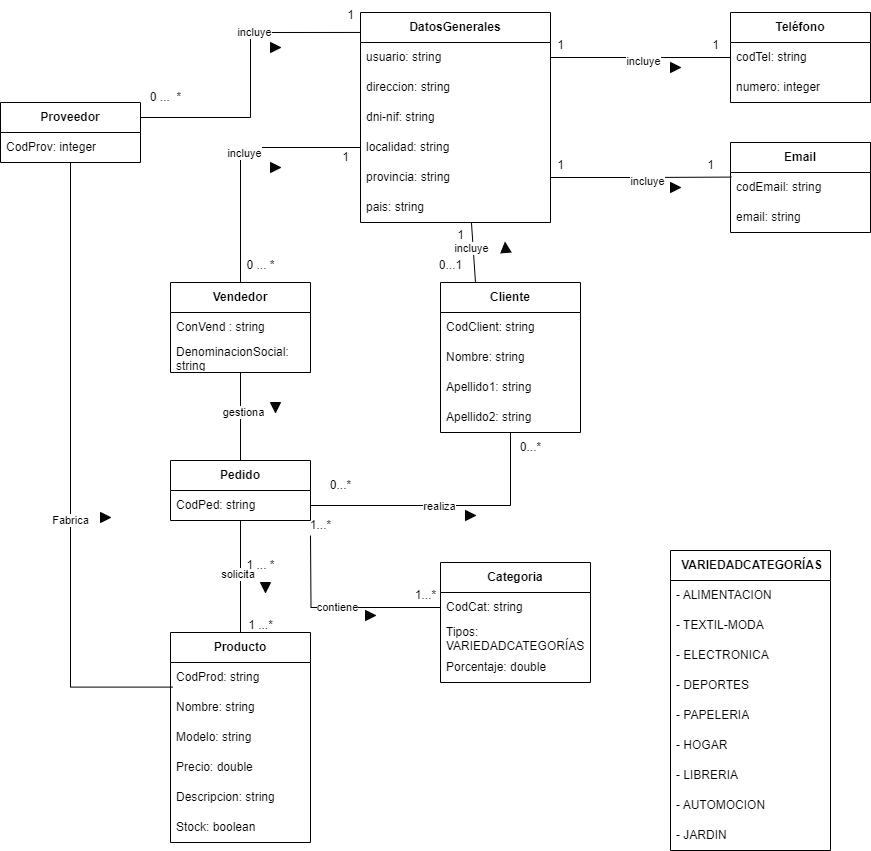
\includegraphics[scale=0.5]{DiagramaClases.png}
\caption{\label{fig:diaClass}Diagrama de clases.}
\end{figure}
\subsection{Diseño de la Base de Datos.}
\subsubsection{Diseño Lógico.}
 Nuestro diseño de bases de datos empezó siendo muy ambicioso (ver figura \ref{fig:bsdini}), finalmente ha quedado mucho más reducida.

\begin{figure}[h]
\centering
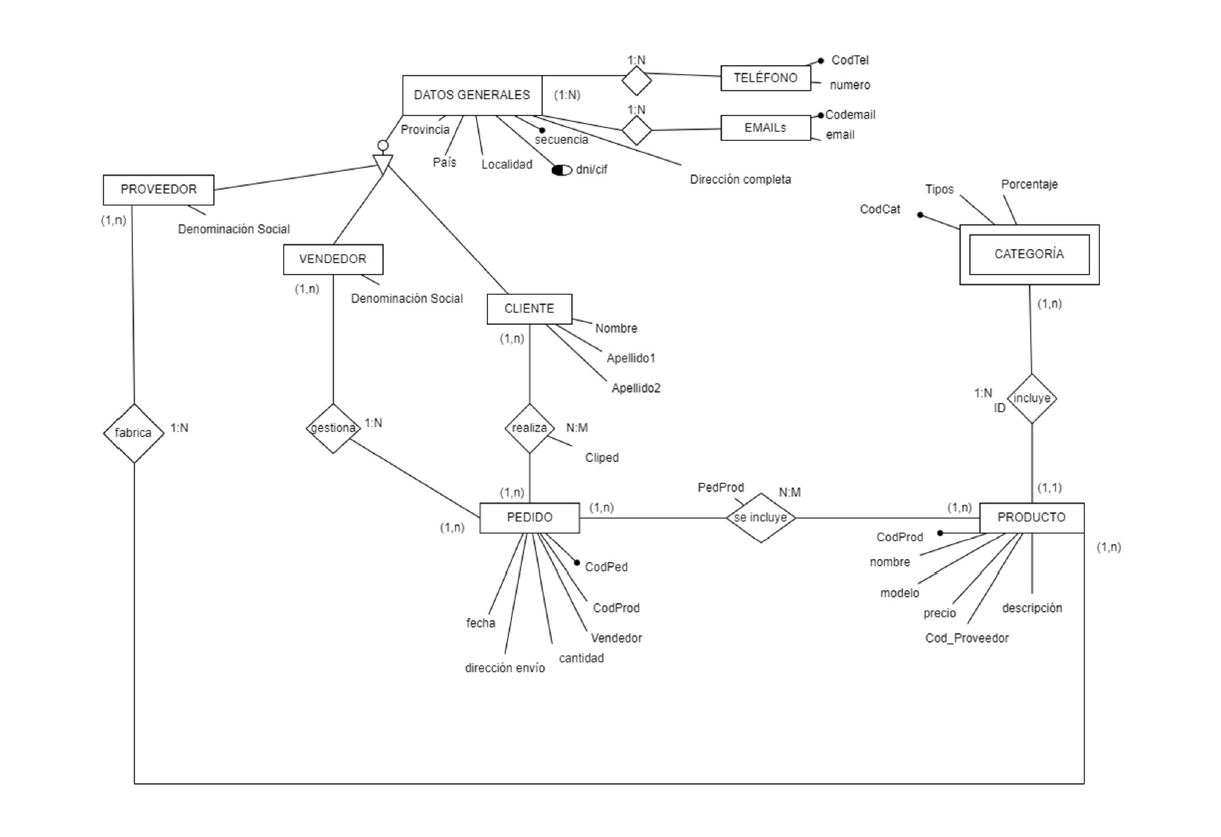
\includegraphics[scale=0.5]{IdeainicialBSD.png}
\caption{\label{fig:bsdini} Diseño de Base de Datos inicial.}
\end{figure}
Entidades, atributos, claves primarias, identificadores únicos, relaciones entre las entidades.
\subsubsection{Diseño Conceptual.}
Tablas, campos, tipos de datos, restricciones, claves primarias, claves foráneas, triggers de validadación si los hubiera.
\subsection{Diseño de la Interfaz.}
En este apartado se define cual va a ser la apariencia visual de la aplicación:  interfaz visual entre el usuario y la aplicación.
En este apartado se debe explicar cómo son las plantillas en las que se basa la apariencia de nuestra interfaz así como cada una de las pantallas que tengamos.

\section{Implementación}
\subsection{Introducción}
En este momento ya se encuentra definido el problema y la solución, por lo que lo siguiente será transformar el modelo obtenido en las actividades anteriores en código fuente.
\subsection{Arquitectura Cliente/Servidor}
Explicar en qué consiste
\subsection{Lenguajes de Programación.}
El lenguaje de programación principal utilizado en este proyecto es PHP, después hemos utilizado plantillas BLADE, también se incluye Javascript, Latex y como lenguaje de marcas HTML utilizando también CSS.

Hemos optado por PHP porque suponía un reto para el proyecto, puesto que los lenguajes con los que tenemos más preferencia de trabajo son JAVA y PHYTON.

% Explicar un poco cada uno de los lenguajes de programación que has utilizado para la realización de tu proyecto.
\subsection{Herramientas de Desarrollo}
Explicar que herramientas has utilizado para desarrollar tu aplicación
\subsection{Codificación}
Todo el código y la información se encuentran ubicados en GitHub, se puede acceder a través de \textit{\url{https://github.com/ymorzam328/KnowBuySell.git}}.\\
% Todo el código desarrollado se encuentra disponible en el pendrive / moodle que se adjunta con esta memoria (a determinar por el departamento de informática).
% \section{Pruebas de software}
% \subsection{Introducción}
% En el desarrollo de cualquier software, una de las actividades asociadas a este proceso es la prueba. En este capítulo se detallarán las pruebas realizadas al software desarrollado. Se intentará valorar la calidad de la aplicación generada, así como detectar y corregir posibles errores. 
% Breve descripción de que son las pruebas del software.

% \subsection{Técnicas de Prueba}
% Explicación de las pruebas de caja blanca y caja negra
% \subsubsection{Pruebas de caja blanca o enfoque estructural}
% Explicar qué son y en qué consisten este tipo de pruebas.
% Nota: en caso de proyectos amplios es posible que no se realice documentación sobre ninguna de estas pruebas puesto que la documentación de las mismas sería muy tediosa. Menciona los aspectos que se han tenido en cuenta en caso de estar en esta situación.
% \subsubsection{Pruebas de caja negra o enfoque funcional}
% Explicar qué son y en qué consisten este tipo de pruebas.
% Estas pruebas se realizan tras la fase de codificación y nos van a determinar si el requisito de una aplicación es parcial o completamente satisfactoria.
% Puedes aplicar pruebas mediante JUnit. Si tu programa es muy grande pon las que te resulten más importantes.

\section{Conclusiones}
\subsection{Resumen de conclusiones}
Ver en Anexo 1 a este documento, donde también se pueden encontrar las Referencias o Bibliografía utilizada.
% \subsection{Propuestas Futuras (opcional)}
% Ampliaciones y/o mejoras que podrías añadir a tu proyecto en un futuro.






% NOTAS INTERNAS PARA TENER EN CUENTA EN EL LATEX NO OLVIDAR BORRAR ANTES DE ENTREGAR
% PRUEBAS PARA AÑADIR COSAS
% \begin{figure}
% \centering
% \includegraphics[width=0.25\linewidth]{frog.jpg}
% \caption{\label{fig:frog}This frog was uploaded via the file-tree menu.}
% \end{figure}

% \subsection{How to add Tables}

% Use the table and tabular environments for basic tables --- see Table~\ref{tab:widgets}, for example. For more information, please see this help article on \href{https://www.overleaf.com/learn/latex/tables}{tables}. 

% \begin{table}
% \centering
% \begin{tabular}{l|r}
% Item & Quantity \\\hline
% Widgets & 42 \\
% Gadgets & 13
% \end{tabular}
% \caption{\label{tab:widgets}An example table.}
% \end{table}

% \subsection{How to add Comments and Track Changes}

% Comments can be added to your project by highlighting some text and clicking ``Add comment'' in the top right of the editor pane. To view existing comments, click on the Review menu in the toolbar above. To reply to a comment, click on the Reply button in the lower right corner of the comment. You can close the Review pane by clicking its name on the toolbar when you're done reviewing for the time being.

% Track changes are available on all our \href{https://www.overleaf.com/user/subscription/plans}{premium plans}, and can be toggled on or off using the option at the top of the Review pane. Track changes allow you to keep track of every change made to the document, along with the person making the change. 

% \subsection{How to add Lists}

% You can make lists with automatic numbering \dots

% \begin{enumerate}
% \item Like this,
% \item and like this.
% \end{enumerate}
% \dots or bullet points \dots
% \begin{itemize}
% \item Like this,
% \item and like this.
% \end{itemize}

% \subsection{How to write Mathematics}

% \LaTeX{} is great at typesetting mathematics. Let $X_1, X_2, \ldots, X_n$ be a sequence of independent and identically distributed random variables with $\text{E}[X_i] = \mu$ and $\text{Var}[X_i] = \sigma^2 < \infty$, and let
% \[S_n = \frac{X_1 + X_2 + \cdots + X_n}{n}
%       = \frac{1}{n}\sum_{i}^{n} X_i\]
% denote their mean. Then as $n$ approaches infinity, the random variables $\sqrt{n}(S_n - \mu)$ converge in distribution to a normal $\mathcal{N}(0, \sigma^2)$.


% \subsection{How to change the margins and paper size}

% Usually the template you're using will have the page margins and paper size set correctly for that use-case. For example, if you're using a journal article template provided by the journal publisher, that template will be formatted according to their requirements. In these cases, it's best not to alter the margins directly.

% If however you're using a more general template, such as this one, and would like to alter the margins, a common way to do so is via the geometry package. You can find the geometry package loaded in the preamble at the top of this example file, and if you'd like to learn more about how to adjust the settings, please visit this help article on \href{https://www.overleaf.com/learn/latex/page_size_and_margins}{page size and margins}.

% \subsection{How to change the document language and spell check settings}

% Overleaf supports many different languages, including multiple different languages within one document. 

% To configure the document language, simply edit the option provided to the babel package in the preamble at the top of this example project. To learn more about the different options, please visit this help article on \href{https://www.overleaf.com/learn/latex/International_language_support}{international language support}.

% To change the spell check language, simply open the Overleaf menu at the top left of the editor window, scroll down to the spell check setting, and adjust accordingly.

% \subsection{How to add Citations and a References List}

% You can simply upload a \verb|.bib| file containing your BibTeX entries, created with a tool such as JabRef. You can then cite entries from it, like this: \cite{greenwade93}. Just remember to specify a bibliography style, as well as the filename of the \verb|.bib|. You can find a \href{https://www.overleaf.com/help/97-how-to-include-a-bibliography-using-bibtex}{video tutorial here} to learn more about BibTeX.

% If you have an \href{https://www.overleaf.com/user/subscription/plans}{upgraded account}, you can also import your Mendeley or Zotero library directly as a \verb|.bib| file, via the upload menu in the file-tree.

% \subsection{Good luck!}

% We hope you find Overleaf useful, and do take a look at our \href{https://www.overleaf.com/learn}{help library} for more tutorials and user guides! Please also let us know if you have any feedback using the Contact Us link at the bottom of the Overleaf menu --- or use the contact form at \url{https://www.overleaf.com/contact}.

% \bibliographystyle{alpha}
% \bibliography{sample}

\end{document}